\section{Metropolis Hastings} 

  Say that with initial distribution $p(\theta)$, we have calculated the posterior as
  \begin{equation}
    p(\theta\,|\,x) \propto p(\theta) \; p(x\,|\,\theta)
  \end{equation}

  It is often the case that the set of possible values of $\theta$ is very large, so it is computationally inefficient to compute the normalizing factor
  \begin{equation}
    p(x) = \sum_\theta p(\theta) \; p(x\,|\,\theta)
  \end{equation}

  Therefore, we only have this function $f(\theta) = p(\theta) \; p(x\,|\,\theta)$ that is directly proportional to $p(\theta\,|\,x)$. That is, we don't know the normalizing constant $c$ such that
  \begin{equation}
    p(\theta\,|\,x) = \frac{f(\theta)}{c}
  \end{equation}

  Using this information, we wish to construct and run an algorithm that converges onto the true posterior distribution $p(\theta\,|\,x)$ at a sufficiently fast rate.

  We begin by constructing a discrete-time irreducible Markov chain with state space $\mathcal{S} = \{1, 2, \ldots, N\}$ representing the set of possible parameter values (the labels for the elements of $\mathcal{S}$ does not matter, since we can construct whatever bijection we want from the actual states to a subset of $\mathbb{N}$). Like a normal Markov chain, we will choose the next state to go to at each step, \textit{but now, we will then choose to accept this proposal to go to that step with an additional probability}. That is, we will construct two matrices:

  \begin{itemize}
    \item An $|\mathcal{S}| \times |\mathcal{S}|$ \textbf{proposal transition matrix} $Q_{prop}$, with
    \begin{equation}
      p(\text{propose } i \mapsto j) = (Q_{prop})_{ij} = q_{prop} (i, j)
    \end{equation}
    being the probability of getting a \textit{proposal} to transition from state $i$ to state $j$. This matrix is constructed by the user and is completely well-defined and known; this choice may also affect the convergence rate. Note that with this formulation, the rows will sum up to $1$ and $Q^T$ is a stochastic matrix. We can also construct $Q_{prop}$ to be symmetric, that is $q_{prop}(i, j) = q_{prop} (j, i)$, for easier calculations.

    \item An $|\mathcal{S}| \times |\mathcal{S}|$ \textbf{acceptance probability matrix} $A$, with
    \begin{align*}
      (\text{accept proposal }i \mapsto j\,|\, \text{propose } i \mapsto j) & = (A)_{ij} = \alpha(i, j) \\
      & = \min \bigg(1, \frac{p(\theta = j \,|\, x)\; q_{prop}(j, i)}{p(\theta = i\,|\, x) \; q_{prop}(i, j)} \bigg) \\
      & = \min\bigg(1, \frac{f(\theta = j) \; q_{prop}(j, i)}{f(\theta = i) \; q_{prop}(i, j)} \bigg) \\
      & = \min\bigg(1, \frac{f(\theta = j)}{f(\theta = i)} \bigg) \;\;\;\;\;\;\; (\text{if } Q_{prop} \text{ symmetric})
    \end{align*}
  \end{itemize}

  Then, we element-wise multiply the two matrices, except the diagonals, to get the \textbf{true transition matrix} $Q$ defined
  \begin{equation}
    (Q)_{ij} = q(i, j) = \begin{cases}
      q_{prop} (i, j) \cdot \alpha (i, j) = q_{prop}(i, j) \cdot \min\bigg(1, \frac{f(\theta = j) \; q(j, i)}{f(\theta = i) \; q(i, j)} \bigg) & \text{ if } i \neq j \\
      1 - \sum_{j \neq i} q(i, j) & \text{ if } i = j
    \end{cases}
  \end{equation}

  where $q(i, j)$ represents the \textbf{true transition probability} of going from state $i$ to state $j$. Note that we have element-wise multiplied every non-diagonal element, and we have defined $(Q)_ii$ such that the sum of each row is $1$ (so that this becomes a viable transition matrix). Note also that this element-wise multiplication makes sense because
  \begin{align*}
    p(\theta_{k+1} = j\,|\, \theta_k = i) & = p(\text{accept proposal }i \mapsto j, \; \text{propose } i \mapsto j) \\
    & = p(\text{accept proposal }i \mapsto j\,|\, \text{propose } i \mapsto j)\; p(\text{propose } i \mapsto j) \\
    & = \alpha(i, j) \cdot q_{prop} (i, j)
  \end{align*}

  This is the Markov chain we wish to get, where "one" step is really a two-step process of proposing and accepting/rejecting. We wish to get the steady state distribution $\pi(\theta)$ of this chain, which can be found in two well-known ways:
  \begin{itemize}
    \item Calculate the left-eigenvector of $Q$ with eigenvalue $1$.
    \item Randomly initialize $\theta_0$ and run the chain for a sufficiently long time to record where it lands at each step
    \begin{equation}
      \theta_0 = i_0, \theta_1 = i_1, \theta_2 = i_2, \theta_3 = i_3, \ldots, \theta_n = i_n
    \end{equation}
    which can be used to approximate $\pi(\theta)$ by defining
    \begin{equation}
      \pi(\theta = i) = \frac{\text{proportion of states in state } i \text{ in the n-step process}}{n}
    \end{equation}
  \end{itemize}

  Finally, we claim that this steady state distribution $\pi(\theta)$ is precisely the posterior we are looking for: $p(\theta\,|\,x)$.

\subsection{Algorithm}

  Given that we have computed a scalar multiple of a high dimensional posterior $\pi = \frac{f}{c}$ defined in $\mathbb{R}^n$ for $n >> 1$, we would like to either optimize $f$ or sample from $f$ to find its true normalizing factor $c$. There are some overlaps in the methods used to achieve these goals. Let us denote our (parameter) state as $\theta \in \mathbb{R}^n$, with a discrete time step denoted by $t$ and step size $h$. 

  Markov Chain Monte Carlo algorithms are extremely simple and computationally efficient, since they only require to compute $f(\theta)$, without any gradient information. They generate a sequence of correlated samples which on the long run converge to a sequence of independent samples. The degree of correlation of nearby samples is called the \textit{autocorrelation} of the MCMC sampler. We first generate a proposal step according to some kernel and then decide whether to accept or reject that proposal. Usually, we have a series of "burn-in" steps that allow the chain to first converge to a local maximum, which we can then throw away. The simplest version of this is with an isotropic Gaussian kernel. 

  \begin{algorithm}
    \caption{Random Walk Metropolis Hastings w/ Isotropic Gaussian Kernel}\label{alg:metropolis_gaussian}
    \begin{algorithmic}

    \Require Initial $\boldsymbol{\theta}_0$, Stepsize $h$, Burn-in steps $\mathcal{B}$

    \For{$t = 0$ to $T$}
        \State $\epsilon_t \sim \mathcal{N}(0, I)$ 
        \State $P_{t+1} \gets \theta_t + \epsilon_t$
        \If{$f(P_{t+1}) \geq f(\theta_t)$}
            \State $\theta_{t+1} \gets P_{t+1}$ 
        \Else
            \State $\delta \sim \mathrm{Uniform}[0, 1]$
            \If{$\delta < f(P_{t+1}) / f(\theta_t)$}
                \State $\theta_{t+1} \gets P_{t+1}$ 
            \Else 
                \State $\theta_{t+1} \gets \theta_t$
            \EndIf
        \EndIf
    \EndFor

    \State Delete first $\mathcal{B}$ states of $\boldsymbol{\theta} = [\theta_0, \theta_1, \ldots, \theta_T]$

    \end{algorithmic}
  \end{algorithm}

  Note that the step size is very important here: If $h$ is too small, then this chain would behave like a random walk. If $h$ it too big, then this chain would mainly stay at one state. Ideally, the acceptance probability should be between $0.2$ and $0.7$. 

  This isotropic MH is not robust, since it would not work well if some parameters of $\theta$ are correlated and the estimated covariance of $f$ at some local maximum is more "diagonal." Therefore, some adaptive mechanism is needed, which we can implement by estimating the covariance matrix of the proposal kernel using the empirical covariance of the proposal steps. To reduce memory allocation, we should use a recursive algorithm to compute the mean and covariance, rather than having to store all the $\theta_t$'s. To maintain stability, we may start adapting after a certain number of steps $B$ and compute covariance estimates every $U$ steps. 

  \begin{algorithm}
    \caption{Adaptive Random Walk Metropolis}\label{alg:adaptive_metro}
    \begin{algorithmic}

    \Require Initial $\boldsymbol{\theta}_0$, Stepsize $h$, Burn-in steps $\mathcal{B}$, Adaptation burn-in $B$, Adaptation frequency $U$
    \State $\mu_0^\mathrm{emp} \gets 0$ 
    \State $\Sigma_0 \gets I$
    \State $\Sigma^\mathrm{emp}_0 \gets I$

    \For{$t = 0$ to $T$}
        \State $\epsilon_t \sim \mathcal{N}(0, \Sigma_t)$ 
        \State $P_{t+1} \gets \theta_t + \epsilon_t$
        \If{$f(P_{t+1}) \geq f(\theta_t)$}
            \State $\theta_{t+1} \gets P_{t+1}$ 
        \Else
            \State $\delta \sim \mathrm{Uniform}[0, 1]$
            \If{$\delta < f(P_{t+1}) / f(\theta_t)$}
                \State $\theta_{t+1} \gets P_{t+1}$ 
            \Else 
                \State $\theta_{t+1} \gets \theta_t$
            \EndIf
        \EndIf
        
        \State $\Sigma^\mathrm{emp}_{t+1} \gets \frac{1}{t+1} \big[(\theta^{t+1} - \mu_t) (\theta^{t+1} - \mu_t)^T - \Sigma^\mathrm{emp}_t \big]$
        \State $\mu_{t+1}^{\mathrm{emp}} \gets \mu_t + \frac{1}{t+1} [ \theta_{t+1} - \mu_t ]$
        
        \If{$t > B$ and $t$ is divisible by $U$} 
            \State $\Sigma_{t+1} \gets \Sigma^\mathrm{emp}_{t+1}$
        \EndIf
    \EndFor

    \State Delete first $\mathcal{B}$ states of $\boldsymbol{\theta} = [\theta_0, \theta_1, \ldots, \theta_T]$

    \end{algorithmic}
  \end{algorithm}

  On top of this even, we can precondition the initial $\Sigma_0$ to be some other estimate of the posterior and weight it accordingly so that our proposal covariance is some "balance" of this computed estimate and the empirical estimate, using a damping parameter $\alpha$. 
  \begin{equation}
    \Sigma_t = \alpha \Sigma_0 + (1 - \alpha) \Sigma^{\mathrm{emp}}, \;\;\;\;\; 0 \leq \alpha \leq 1
  \end{equation}

  The lower the $\alpha$, the more the precomputed estimate is "washed away" by the empirical covariance. We can also treat the $\alpha$ as a variable function $\alpha(t)$ and adapt its value as the chain runs. For example, if we would like the precomputed covariance to have more weight in the beginning (for stability), but eventually completely overpowered by the empirical covariance, we can choose it such that $\alpha(0) = 1$ and $\alpha \rightarrow 0$ as $t \rightarrow +\infty$, with the specific behavior customized to the problem. 

  \begin{algorithm}
    \caption{Adaptively Preconditioned Random Walk Metropolis}\label{alg:adaptive_precon_metro}
    \begin{algorithmic}

    \Require Initial $\boldsymbol{\theta}_0$, Stepsize $h$, Burn-in steps $\mathcal{B}$, Adaptation burn-in $B$, Adaptation frequency $U$, Damping function $\alpha$, Precomputed covariance estimate $\Sigma^{\mathrm{pre}}$
    \State $\mu_0^\mathrm{emp} \gets 0$ 
    \State $\Sigma^\mathrm{emp}_0 \gets I$
    \State $\Sigma_0 \gets I$

    \For{$t = 0$ to $T$}
        \State $\epsilon_t \sim \mathcal{N}(0, \Sigma_t)$ 
        \State $P_{t+1} \gets \theta_t + \epsilon_t$
        \If{$f(P_{t+1}) \geq f(\theta_t)$}
            \State $\theta_{t+1} \gets P_{t+1}$ 
        \Else
            \State $\delta \sim \mathrm{Uniform}[0, 1]$
            \If{$\delta < f(P_{t+1}) / f(\theta_t)$}
                \State $\theta_{t+1} \gets P_{t+1}$ 
            \Else 
                \State $\theta_{t+1} \gets \theta_t$
            \EndIf
        \EndIf
        
        \State $\Sigma^\mathrm{emp}_{t+1} \gets \frac{1}{t+1} \big[(\theta^{t+1} - \mu_t) (\theta^{t+1} - \mu_t)^T - \Sigma^\mathrm{emp}_t \big]$
        \State $\mu_{t+1}^\mathrm{emp} \gets \mu_t + \frac{1}{t+1} [ \theta_{t+1} - \mu_t ]$
        
        \If{$t > B$ and $t$ is divisible by $U$} 
            \State $\Sigma_{t+1} \gets \alpha(t) \cdot \Sigma^\mathrm{pre} + (1 - \alpha(t)) \cdot \Sigma^\mathrm{emp}_{t+1}$
        \EndIf
    \EndFor
    \State Delete first $\mathcal{B}$ states of $\boldsymbol{\theta} = [\theta_0, \theta_1, \ldots, \theta_T]$

    \end{algorithmic}
  \end{algorithm}

\subsection{Detailed Balance: Justification of the Metropolis Algorithm}

  But why does $\pi(\theta) = p(\theta\,|\,x)$? Given a Markov chain $\theta_0$ with transition matrix $Q$, the chain is said to satisfy \textbf{detailed balance} with respect to a distribution $\pi(\theta)$ if
  \begin{equation}
    \pi(\theta = i) q(i, j) = \pi(\theta = j) q(j, i)
  \end{equation}

  for all $i, j \in \mathcal{S}$. In fact, we claim that $\theta_i$ does satisfy detailed balance with respect to $p(\theta\,|\,x)$. That is, it satisfies
  \begin{equation}
    p(\theta = i\,|\,x) q(i, j) = p(\theta = j\,|\,x) q(j, i)
  \end{equation}

  This case is trivial for when $i=j$, so assume $i \neq j$. A transition from $i$ to a different $j$ can only be achieved with an accepted proposed step, which happens with probability
  \begin{align*}
    q(i, j) & = q_{prop} (i, j) \cdot \alpha(i, j) \\
    & = q_{prop} (i, j) \cdot \min\bigg( 1, \frac{p(\theta = j\,|\,x)\; q_{prop} (j, i)}{p(\theta = i\,|\,x) \; q_{prop}(i, j)}\bigg) \\
    & = \frac{q_{prop} (i, j)}{p(\theta = i\,|\,x)} \min\big( p(\theta = i\,|\,x), \frac{p(\theta = j\,|\,x)\; q_{prop} (j, i)}{q_{prop}(i, j)} \big) \\
    & = \frac{1}{p(\theta = i\,|\,x)} \min \big( p(\theta = i\,|\,x)\; q_{prop} (i, j), p(\theta = j\,|\,x) \; q_{prop} (j, i) \big)
  \end{align*}

  Applying the same method from transitioning from $j$ to $i$ gives the same equation, but with the $i$ and $j$'s switched.
  \begin{equation}
    q(j, i) = \frac{1}{p(\theta = j\,|\,x)} \min \big( p(\theta = j\,|\,x)\; q_{prop} (j, i), p(\theta = i\,|\,x) \; q_{prop} (i, j) \big)
  \end{equation}

  But switching the $i$ and $j$ leaves the terms inside the minimum invariant. Therefore, we can see that
  \begin{equation}
    p(\theta = i\,|\,x)\; q(i, j) = \min \big( p(\theta = j\,|\,x)\; q_{prop} (j, i), p(\theta = i\,|\,x) \; q_{prop} (i, j) \big) = p(\theta = j\,|\,x)\; q(j, i)
  \end{equation}

  proving detailed balance. Now, we can sum the left hand side of the detailed balance equation over $i$ to get
  \begin{equation}
    \sum_i p(\theta = i\,|\,x) q(i, j) = \sum_i p(\theta = j\,|\,x) q(j, i) = p(\theta = j\,|\,x) \sum_i q(j, i) = p(\theta = j\,|\,x)
  \end{equation}

  which in matrix form, says
  \begin{equation}
    p(\theta\,|\,x) Q = p(\theta\,|\,x)
  \end{equation}

  where $p(\theta\,|\,x) = \big( p(\theta=1\,|\,x) \ldots p(\theta=N\,|\,x)\big)$ and $Q_{ij} = q(i, j)$. This implies that $p(\theta\,|\,x)$ is a stationary distribution, and therefore, computing the stationary distribution is equivalent to computing $p(\theta\,|\,x)$.

  The intuition behind detailed balance is quite easy to understand, too. Suppose we start a chain in the stationary distribution, so that the respective probabilities $\theta_0 \sim \pi(\theta)$ of starting at position are "smeared" across all states $i$. Then, the quantity $\pi(\theta = i) q (i, j)$ represents the "amount" of probability that flows down edge $i \rightarrow j$ in one time step. If detailed balance holds, then the amount of probability flowing from $i \rightarrow j$ equals the amount that flows from $j \rightarrow i$ (which is $\pi(\theta = j) q(j, i)$). Therefore, there is no \textit{net} flux of probability along the edge $i \leftrightarrow j$ during one time step (remember this holds only for when the chain is in the stationary distribution).

  \begin{figure}[H]
    \centering
    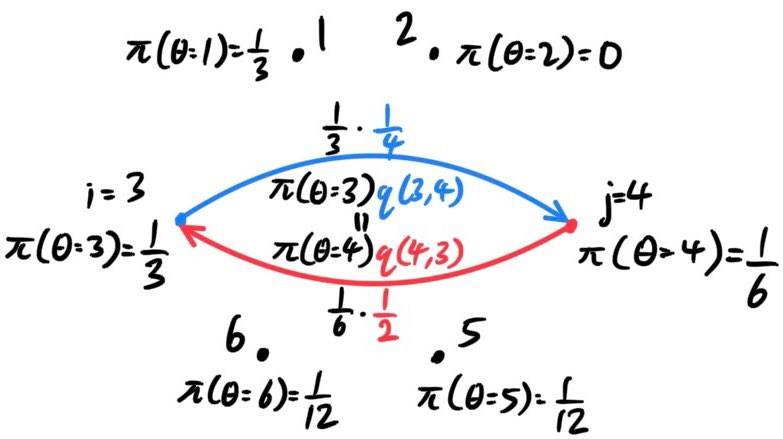
\includegraphics[width=0.5\textwidth]{img/Detailed_Balance.jpg}
    \caption{Visualization of detailed balance in Markov chain}
  \end{figure}

\subsection{Metropolis-Hastings: Example}

  Suppose we want a Markov chain of state space $\mathcal{S} = \{1, 2\}$ with the steady state distribution
  \begin{equation}
    \pi = \begin{pmatrix} \frac{3}{4} & \frac{1}{4} \end{pmatrix} \iff \pi(\theta = 1) = \frac{3}{4}, \; \pi(\theta = 2) = \frac{1}{4}
  \end{equation}

  To implement the Metropolis-Hastings algorithm, we calculate the proposal matrix and acceptance matrix
  \begin{equation}
    Q_{prop} = \begin{pmatrix} \frac{1}{2} & \frac{1}{2} \\ \frac{1}{2} & \frac{1}{2} \end{pmatrix} \text{ and } 
    A = \begin{pmatrix} 1 & \frac{1}{3} \\ 1 & 1 \end{pmatrix}
  \end{equation}

  which is calculated since $\alpha(1, 2) = \min\big(1, \frac{1/4}{3/4} \big) = 1/3$ and $\alpha(2, 1) = \min \big(1, \frac{3/4}{1/4} \big) = 1$. We multiply the nondiagonal entries together and fill in the diagonals to get
  \begin{equation}
    \begin{pmatrix} & \frac{1}{2} \cdot \frac{1}{3} \\ \frac{1}{2} \cdot 1 & \end{pmatrix} \implies 
    Q = \begin{pmatrix} \frac{5}{6} & \frac{1}{6} \\ \frac{1}{2} & \frac{1}{2} \end{pmatrix}
  \end{equation}

  Which can be visualized as an object jumping between two nodes with the following transitions.

  \begin{figure}[H]
    \centering
    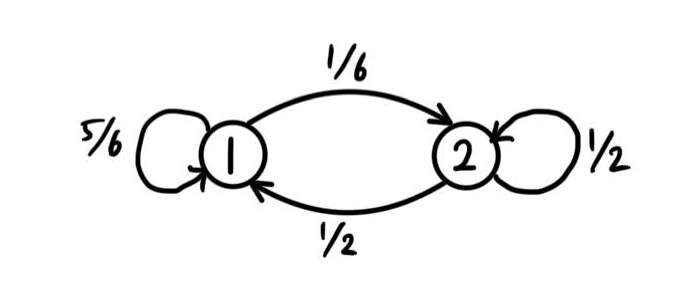
\includegraphics[width=0.5\textwidth]{img/2_state_chain.jpg}
    \caption{Two-state Markov chain with transition probabilities}
  \end{figure}

